\newpage 

\section{Hashing \& Collisions}

In the previous section we lightly touched on the topic of hashing in Definition (\ref{def:hash_table}). 
This section will dive into more detail and difficulties collisions in hashing.

\begin{Def}[Collisions]

    A \textbf{collision} occurs when two different keys hash to the same index in a hash table.
    This is an unavoidable issue in hashing when keys begin to exceed the available indices.
\end{Def}

\begin{figure}[ht!]

    \centering
    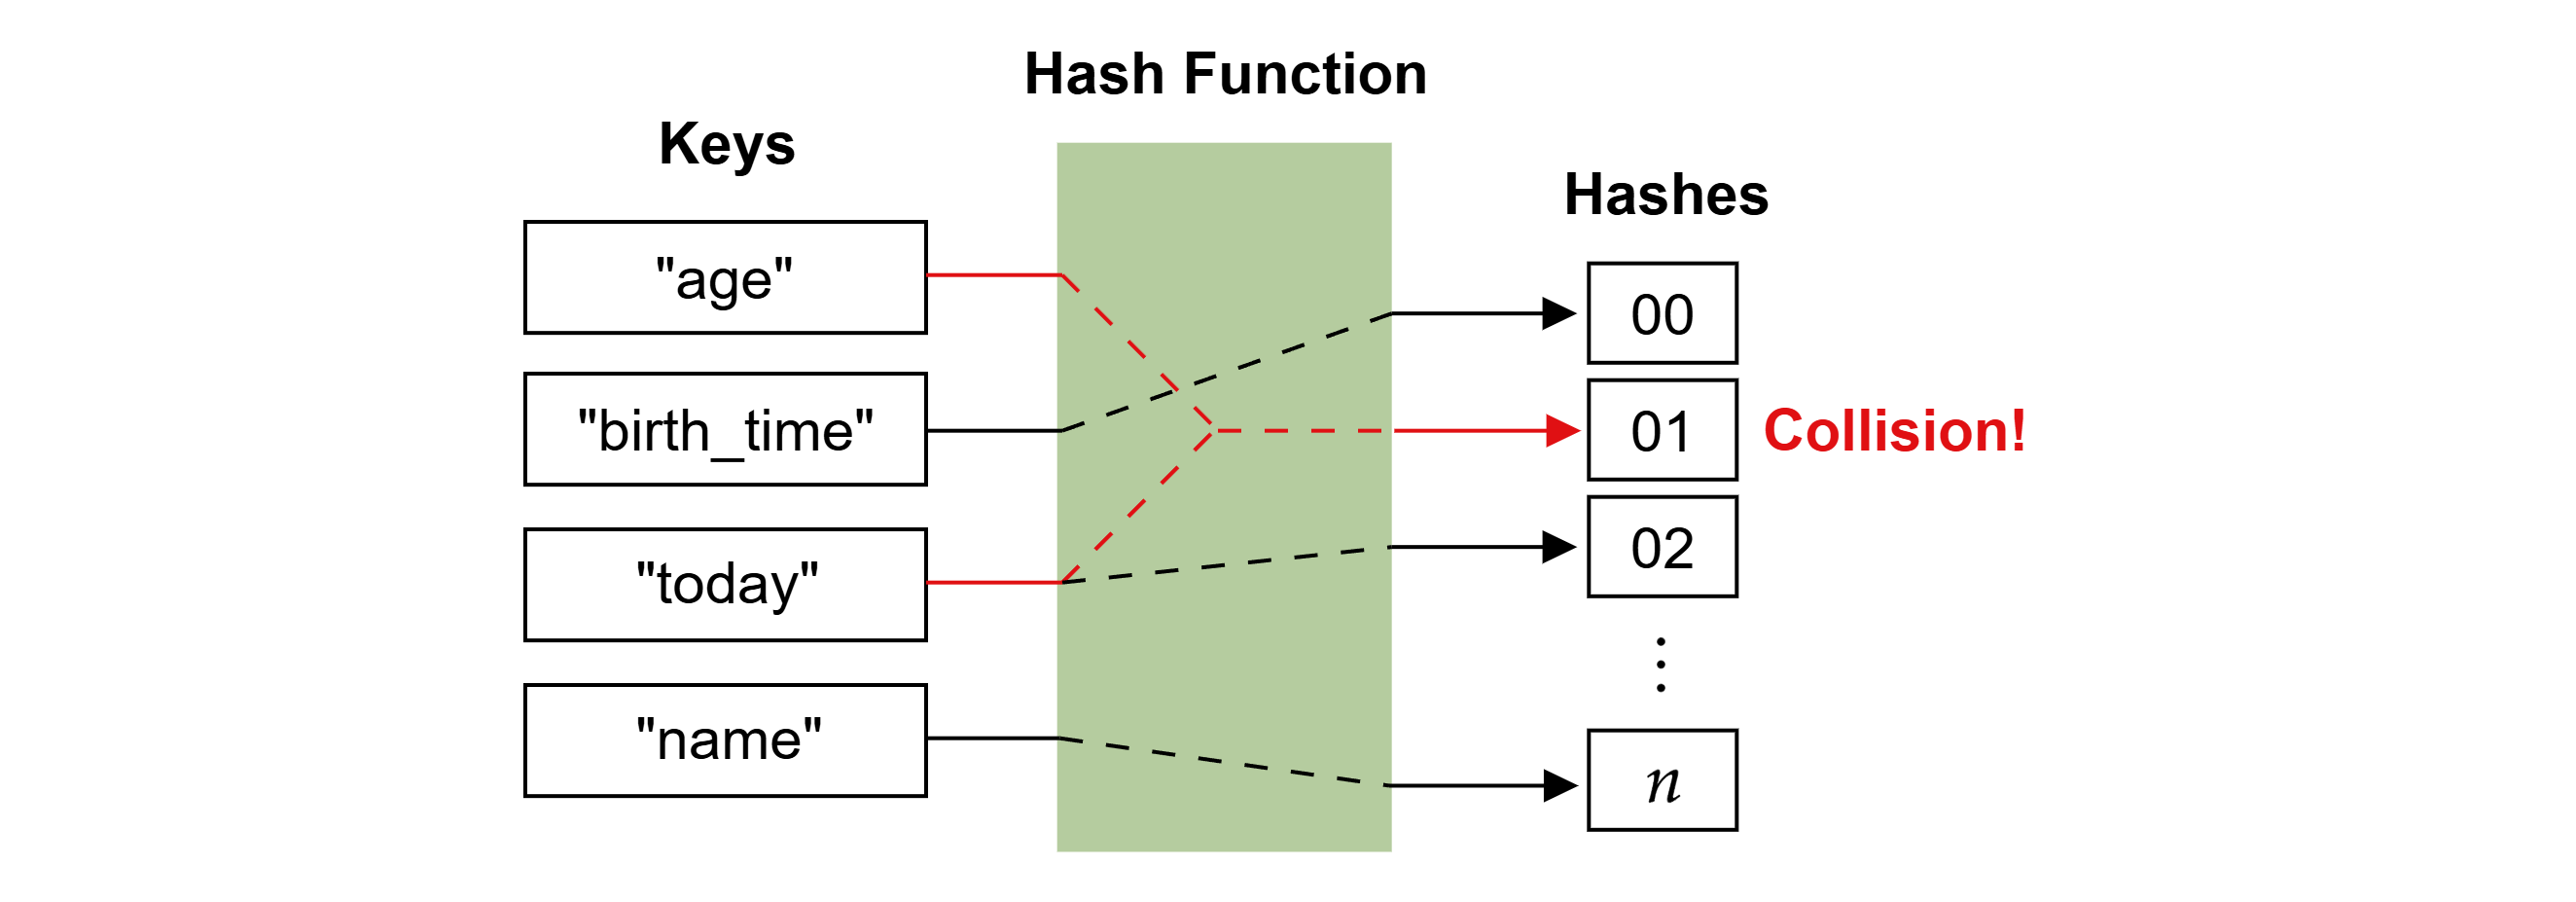
\includegraphics[width=\textwidth]{Sections/hash/collision.png}
    \caption{Four keys (`age', `birth\_time', `today', `name') go through a hash function to $n$ possible indices.
    Keys, `birth\_time' and `name', find a unique one-to-one mapping; However, `age' and `today' both hash to the same index, causing a collision.}
    \label{fig:collision}
\end{figure}
\begin{Example}[Simple Hashing Algorithm]

    Consider the hashing algorithm $H$, it takes the first ASCII value modulo the size 
    of the table. Concretely, $H(k):=\text{ASCII}(k[0])\ \%\ n$, where $n$ is the size of the table.\\

    \noindent
    Given the function $H$, we consider the following keys under a hash table of size $10$:

    \begin{itemize}
        \item \textbf{Key:} `apple' $\rightarrow$ ASCII value $=97$ $\rightarrow$ $H(\text{apple})=97\ \%\ 10 = 7$
        \item \textbf{Key:} `banana' $\rightarrow$ ASCII value $=98$ $\rightarrow$ $H(\text{banana})=98\ \%\ 10 = 8$
        \item \textbf{Key:} `bread' $\rightarrow$ ASCII value $=98$ $\rightarrow$ $H(\text{bread})=98\ \%\ 10 = 8$
    \end{itemize}
    
    \noindent
    Here, we see that `banana' and `bread' both hash to index $8$, causing a collision.
\end{Example}
One could have a superb hashing algorithm, but when space is tight, collisions are inevitable. We'll look at two particular methods for dealing with this issue.

\newpage 

\subsection{Open Addressing}
\noindent
Our first method:
\begin{Def}[Open Addressing]

    \textbf{Open addressing} is a collision resolution method where, upon a collision, the algorithm searches for the next available slot via a probing sequence.\\

    \noindent
    \textbf{Wrap Around:} the algorithm uses a modulo operation (e.g., Given a table size of 10 and request for index 12, the algorithm would use $12\ \%\ 10 = 2$).
    
    \noindent
    \rule{\textwidth}{0.4pt}

    \noindent
    \textbf{Time Complexity:} $O(n)$, where $n$ is the number of elements in the hash table. For example, say the only free index is at 0 with all other
    indices occupied. If we hash to index 1, the algorithm will have to walk all $n$ indices to find the free index at 0. Changing the probe method only switches order of indices checked, not the worst case.\\
    \textbf{Space Complexity:} $O(n)$, where $n$ is the size of the hash table (no additional space).
\end{Def}

\begin{figure}[ht!]

    \centering
    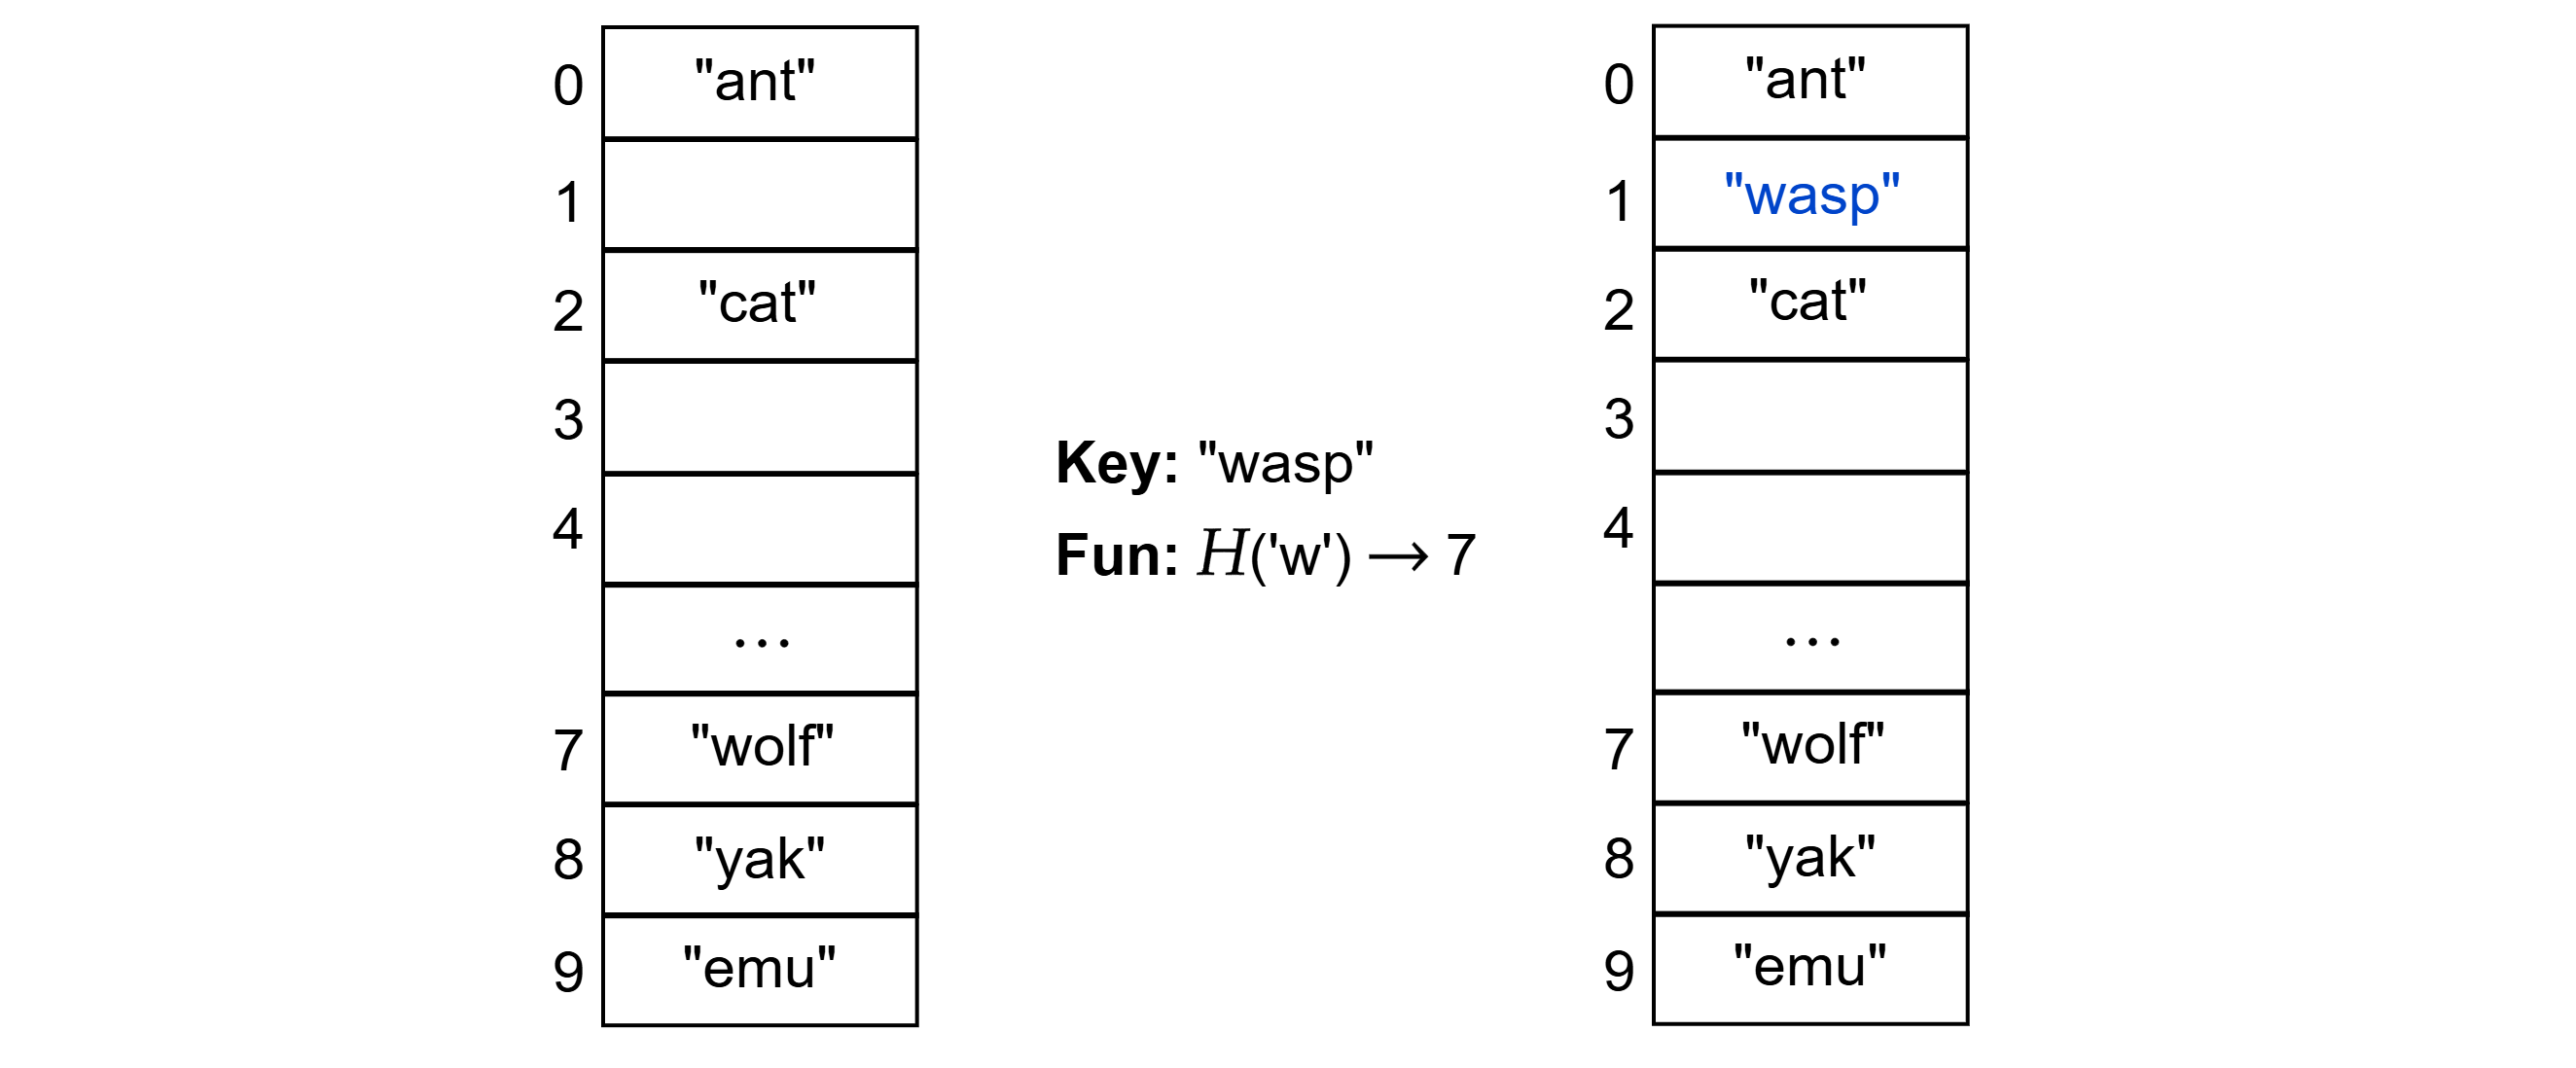
\includegraphics[width=\textwidth]{Sections/hash/open_addressing.png}
    \caption{On the left is an existing hash table of 10 elements filled with various keys. The middle shows the insertion of a new key,
    `wasp', which the function $H$ hashes to index $7$; However, index $7$ already occupied. The algorithm walks through the table, wrapping around
    to the beginning, finding a free index at 1. The right shows the final state of the hash table with `wasp' inserted at index $1$.}
    \label{fig:open_addressing}
\end{figure}

\begin{Def}[Linear Probing]

   \textbf{Linear Probing} in open addressing refers to sequentially checking each index for an available slot (e.g., Figure \ref{fig:open_addressing}).
\end{Def}

\newpage

\begin{Def}[Quadratic Probing]

    Given a universal hashing function  $H(x)$, a \textbf{quadratic probing} resolves collisions by defining,
    \[h(x,k):= (H(x) + k^2)\ \%\ n\] 
    Where $k$ defines the number of collisions, and $n$ hash table size. The algorithm may\\
    \underline{\textbf{never discover}} particular cells due to its even probing style.
    We \textbf{terminate execution} once $n$ indices have been checked, avoiding an infinite loop.
\end{Def}

\noindent
So why even use quadratic probing?
\begin{Def}[Clustering]

    \textbf{Clustering} is a phenomenon in open addressing where multiple keys form contiguous \emph{runs} of occupied indices.
    This degrades linear probing performance; Such is the main motivation behind quadratic probing.
\end{Def}

\begin{figure}[ht!]

    \centering
    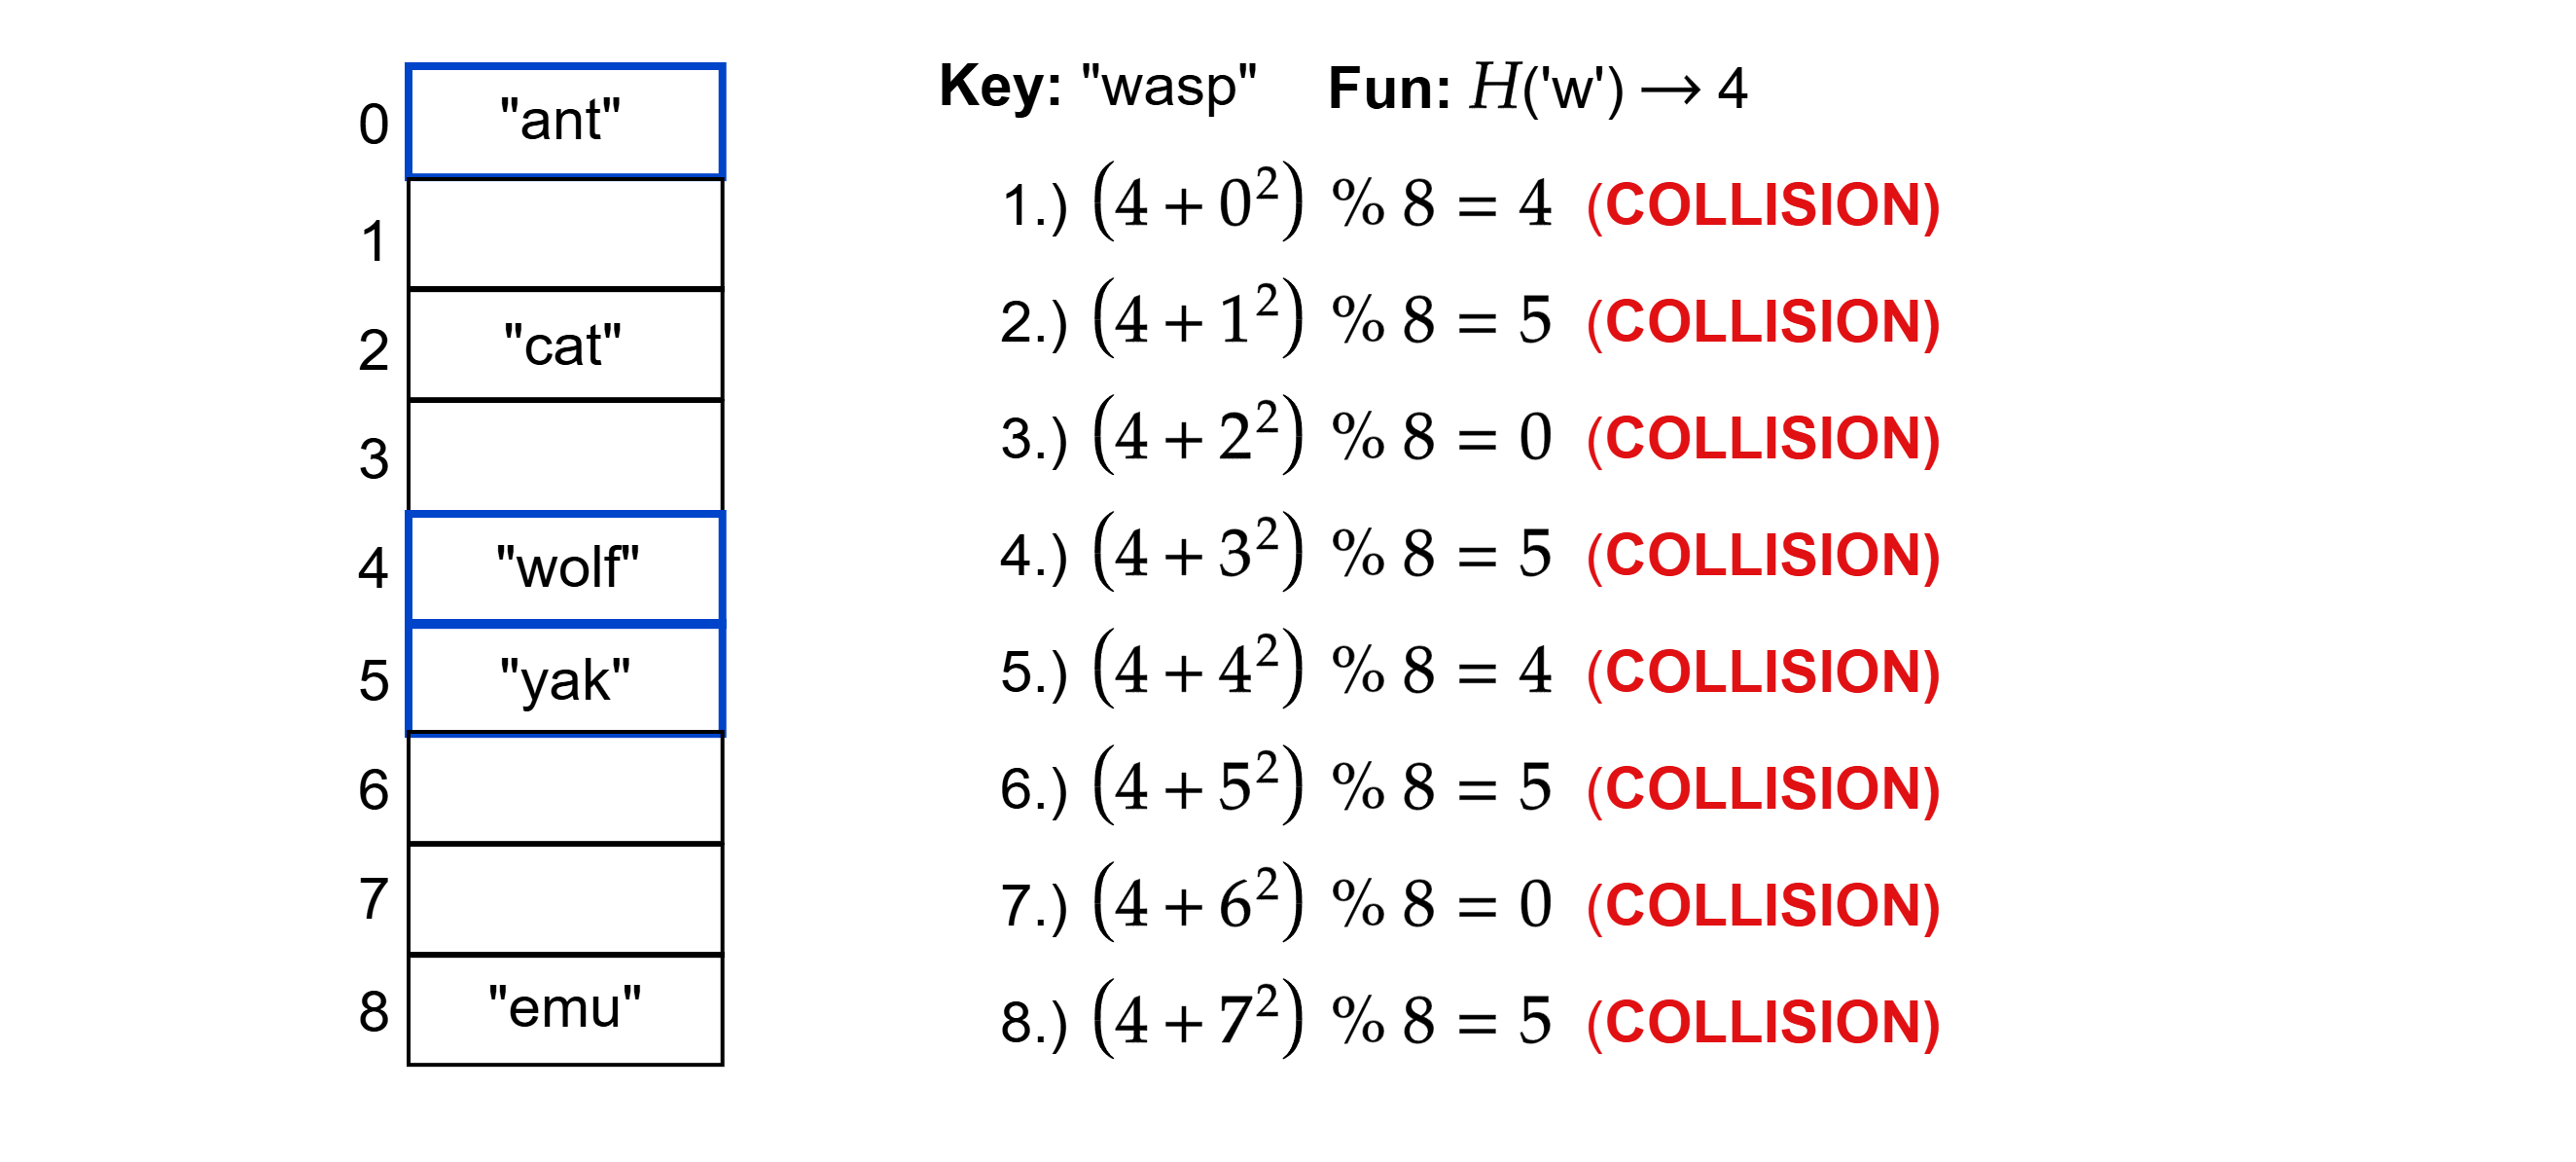
\includegraphics[width=\textwidth]{Sections/hash/quadratic_probing.png}
    \caption{On the left is an existing hash table of 8 elements. We attempt to insert a new key, `wasp', which hashes to index $4$;
    Though, 4 in occupied. The algorithm continues with $(4 + 1^2)\ \%\ 8 = 5$, which is also occupied. After some probing, it appears only indices $4, 5, 0$
    are appearing, from which are all occupied. The algorithm terminates at its $n$-th attempt with $(4+7^2)\ \%\ 8 = 5$. No spaces were found. One could imagine
    that if the table were larger or $0,4,5$ were free, the algorithm would have had better success.}
    \label{fig:quadratic_probing}
\end{figure}

\newpage 

\begin{Def}[Double Hashing]

  \label{def:double_hashing}
  \textbf{Double hashing} resolves collisions by using two hash functions; Given, $H_1(x)$ and $H_2(x)$ uniform hashing functions,
  we define the probe sequence $h(x,k)$ as:
  \[
    h(x,k) := \bigl(H_1(x) + k \cdot H_2(x)\bigr)\ \%\ n,
  \]
  Where $k$ is the collision count, and $n$ is the hash table size.
  $H_2(x)$ is chosen such that:
  \begin{itemize}
    \item The hash satisfies $0 < H_2(x) < n$ (i.e., The result is likely taken by modulo $n$).
    \item It is pair-wise independent from $H_1(x)$ (i.e., not a transformation of/related to $H_1(x)$).
    \item Computationally inexpensive to evaluate.
    \item All outputs of $H_2(x)$ are relatively prime to $n$ (does not share any common factors other than $1$), ensuring all entries are probed.
  \end{itemize}
\end{Def}

\noindent 
We elaborate on the need for relatively prime numbers:
\begin{theo}[Probing Period]
 
    \label{thm:probes_period}
    A \textbf{period} defines the number of unique elements before the sequence begins to repeat. This cycle length is defined as the ratio:
    \[ \dfrac{n}{\gcd(n, H_2(x))} \]
    Where $n$ is the hash table size, and $H_2(x)$ is each hash output on an arbitrary $x$ input. We ideally want $\gcd(n, H_2(x))=1$ 
    for each $x$ to achieve a full period of $n$. Hence, if $n$ is a power of 2,
    $H_2(x)$ may uniformly provide odd numbers; Otherwise, for that particular key, it will only partially probe the table.
\end{theo}

\noindent
Without too much number theory, we attempt to intuitively understand the theorem:
\begin{Proof}[Length of Probing Period]

    \label{proof:probes_period}
    In terms of modulo, $n$ defines a cycle of $n$ elements, $0, 1, \ldots, n-1$; Each element is called a \textbf{residue class} (i.e., all possible remainders).
    E.g., 8 has residue classes 0--7 . Given a finite set of integers $\mathcal{H}$ (i.e., our hash function),
    all $\mathcal{H}_i$ need be co-prime to $n$ to exhaust all residue classes. We exclude all $\mathcal{H}_i \geq n$, as $n$'s cycle is definitively
    over (also by Definition \ref{def:double_hashing}). E.g., $1\ \%\ 8 = 1$, $9\ \%\ 8 = 1$. We pick a fixed-hash $h:=\mathcal{H}_i$ such that $\gcd(n, h) = d > 1$.
    Recall that we calculate $(k \cdot h)\ \%\ n$ for each $k$ collision. Hence if $h$ and $n$ factors intersect at $d$,
    then the $k = n/d_{th}$ collision will produce a multiple of $n$, terminating prematurely at $0$.

\end{Proof}

\newpage 
\noindent
Let's try an example to see how this works:

\begin{Example}[Double Hashing without co-primes]

    Consider a $H_1(x)$ function which always causes collisions, forcing the use the $H_2(x)$ function:
    \[
        H_1(x) := x^0 \quad H_2(x) := x^2\ \%\ (n-1)
    \]
    \noindent
    Giving us the full function:
    \[
    h(x,k) := \bigl(x^0 + k \cdot \left(x^2\ \%\ (n-1)\right)\bigr)\ \%\ n
    \]
    Observe when $n=12$, with key $x=3$, while increasing $k$ collisions:

    \begin{center}
    
 
    \setlength{\tabcolsep}{3pt}
\renewcommand{\arraystretch}{1.1}
\begin{tabular}{r|*{9}{c}}
    \multicolumn{1}{c|}{$
      k \cdot (3^2\ \%\ 11)\ \%\ 12
    $}
      & $h(x,k)$ \\
    \hline
    $0 \cdot 9\ \%\ 12$  & 0 \\
    $1 \cdot 9\ \%\ 12$  & 9   \\
    $2 \cdot 9\ \%\ 12$  & 6   \\
    $3 \cdot 9\ \%\ 12$  & 3   \\
    $4 \cdot 9\ \%\ 12$  & 0   \\
    $5 \cdot 9\ \%\ 12$  & 9   \\
    $6 \cdot 9\ \%\ 12$  & 6   \\
    $7 \cdot 9\ \%\ 12$  & 3   \\
    $8 \cdot 9\ \%\ 12$  & 0   \\
    $9 \cdot 9\ \%\ 12$  & 9   \\
    $10 \cdot 9\ \%\ 12$ & 6   \\
\end{tabular}
     \end{center}
\noindent
Since $\gcd(12, 9) = 3$, the probing period is $12/3 = 4$, only touching indices 
$\{0,3,9,6\}$.

\end{Example}

\subsection{Searching: Insertion \& Deletion}
Things become trickier with a populated hash table with previous 
deletions:

\begin{figure}[ht!]
    \centering
    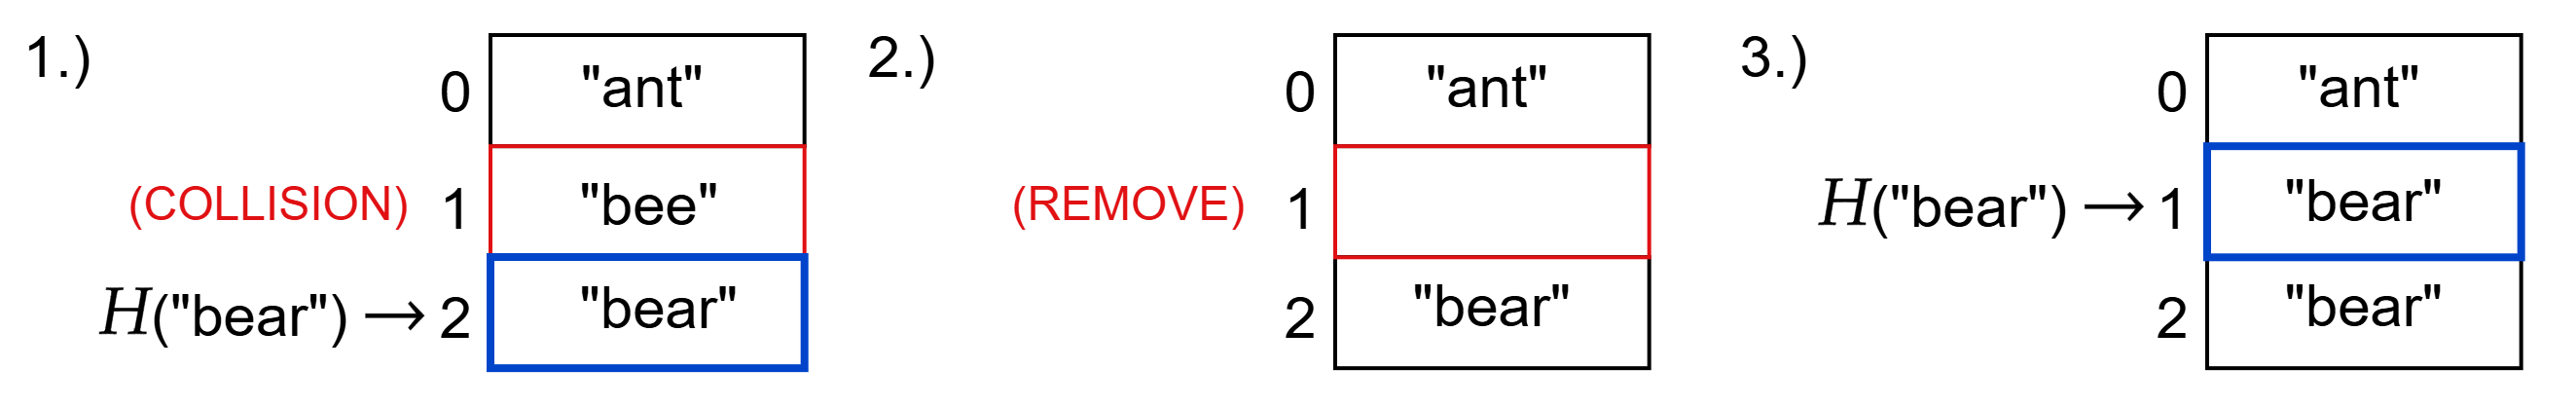
\includegraphics[width=\textwidth]{./Sections/hash/delete.png}
    \caption{Demonstrates complications when inserting into a table blindly. 3.) niaively inserts ``bear'' at index
    1 despite it already existing in the table. This is caused by a previous collision (1) and removal of the collider (2).}
    \label{fig:delete}
\end{figure}

\newpage 

\begin{theo}[Safe Insertion]

    \label{thm:safe_insertion}
    
    To safely insert a key into a hash table, we create three distinctions for each cell:
    \begin{itemize}
        \item \textbf{Empty:} The index is empty, and a key can be inserted.
        \item \textbf{Occupied:} The index is occupied (blocked) by another key.
        \item \textbf{Deleted:} This index was previously occupied but free.
    \end{itemize}

    \noindent
    We may proceed as normal for events Empty and Occupied, but Deleted requires special handling;
    First, take note of the first \textbf{deleted index} then probe the table:
    \begin{itemize}
        \item \textbf{Empty:} If an empty index is found, insert at the first deleted index.
        \item \textbf{Occupied/Deleted:} Continue probing.
        \item \textbf{Duplicate} If the same key is found, insert any data, otherwise terminate.
    \end{itemize}

    \noindent
    Insertion at the first deleted index is safe, as if the key already existed in the table,
    it would have been inserted at any found empty index.
\end{theo}

\begin{figure}[ht!]
    \centering
    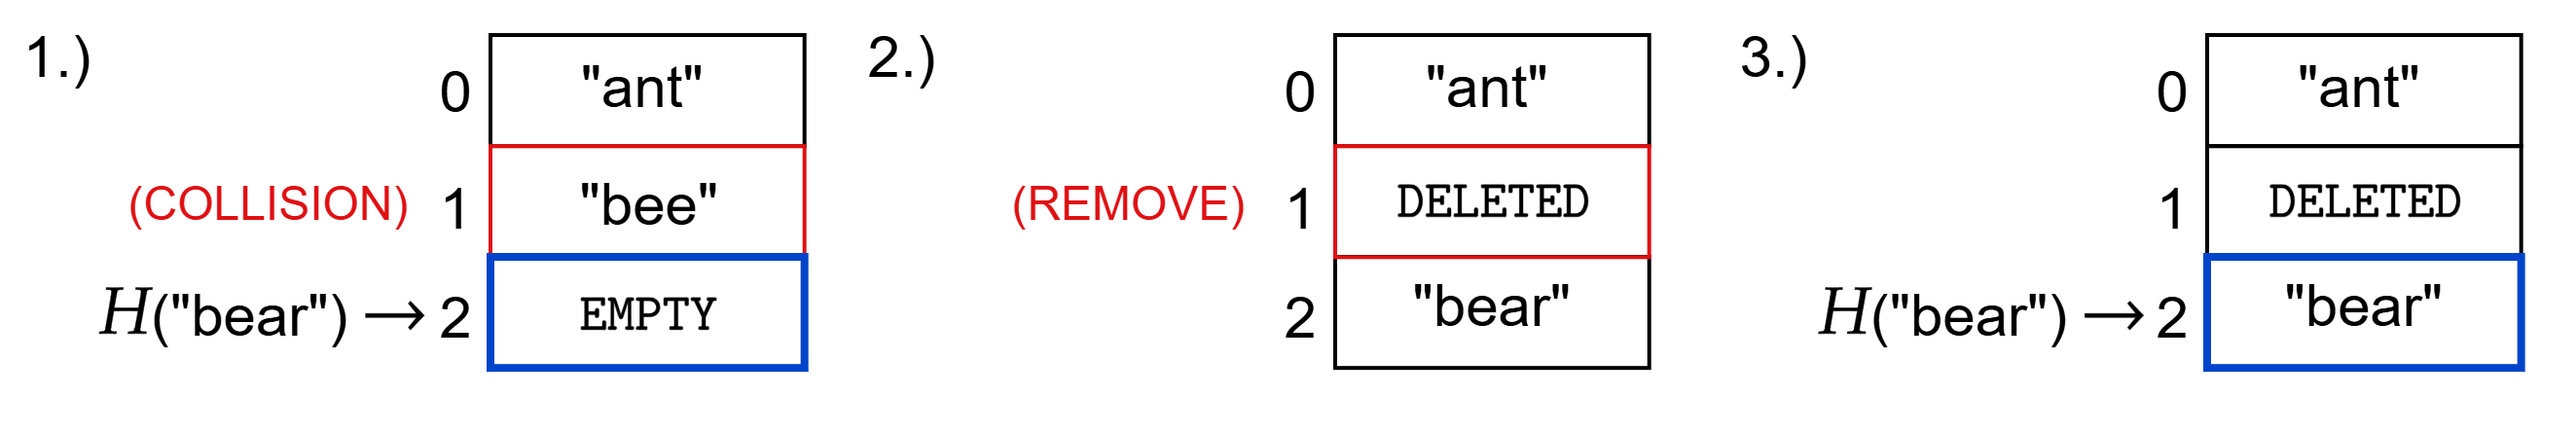
\includegraphics[width=\textwidth]{./Sections/hash/delete_2.png}
    \caption{Revisiting Figure \ref{fig:delete} at (3) we continue to probe after finding a deleted index.
    This leads us to find the already inserted key, ``bear'', at index 2.}
    \label{fig:delete_2}
\end{figure}

\subsection{Separate Chaining \& Linked Lists}

\noindent
A problem we have with open addressing is that it requires a lot of array space; If we run out of space, we have to 
resize the table, \underline{\textbf{which is costly}}:

\begin{theo}[Resizing a Hash Table]

    \label{thm:resize_hash_table}
    Resizing a hash table requires rehashing all keys, which is $O(n)$, where $n$ is the number of elements in the table, 
    excluding the computation cost of hashing each key again.
\end{theo}

\newpage

\noindent
This brings us to the motivation for our second method of collision resolution:

\begin{Def}[Separate Chaining]

    \label{def:separate_chaining}

    \textbf{Separate chaining} is a collision resolution method where each index contains a \textbf{bucket}, which contains 
    all keys that hash to such index. This saves contiguous memory space, as the array can stay a fixed size while holding object
    references living in the heap.
\end{Def}

\vspace{-1em}
\begin{figure}[ht!]

    \centering
    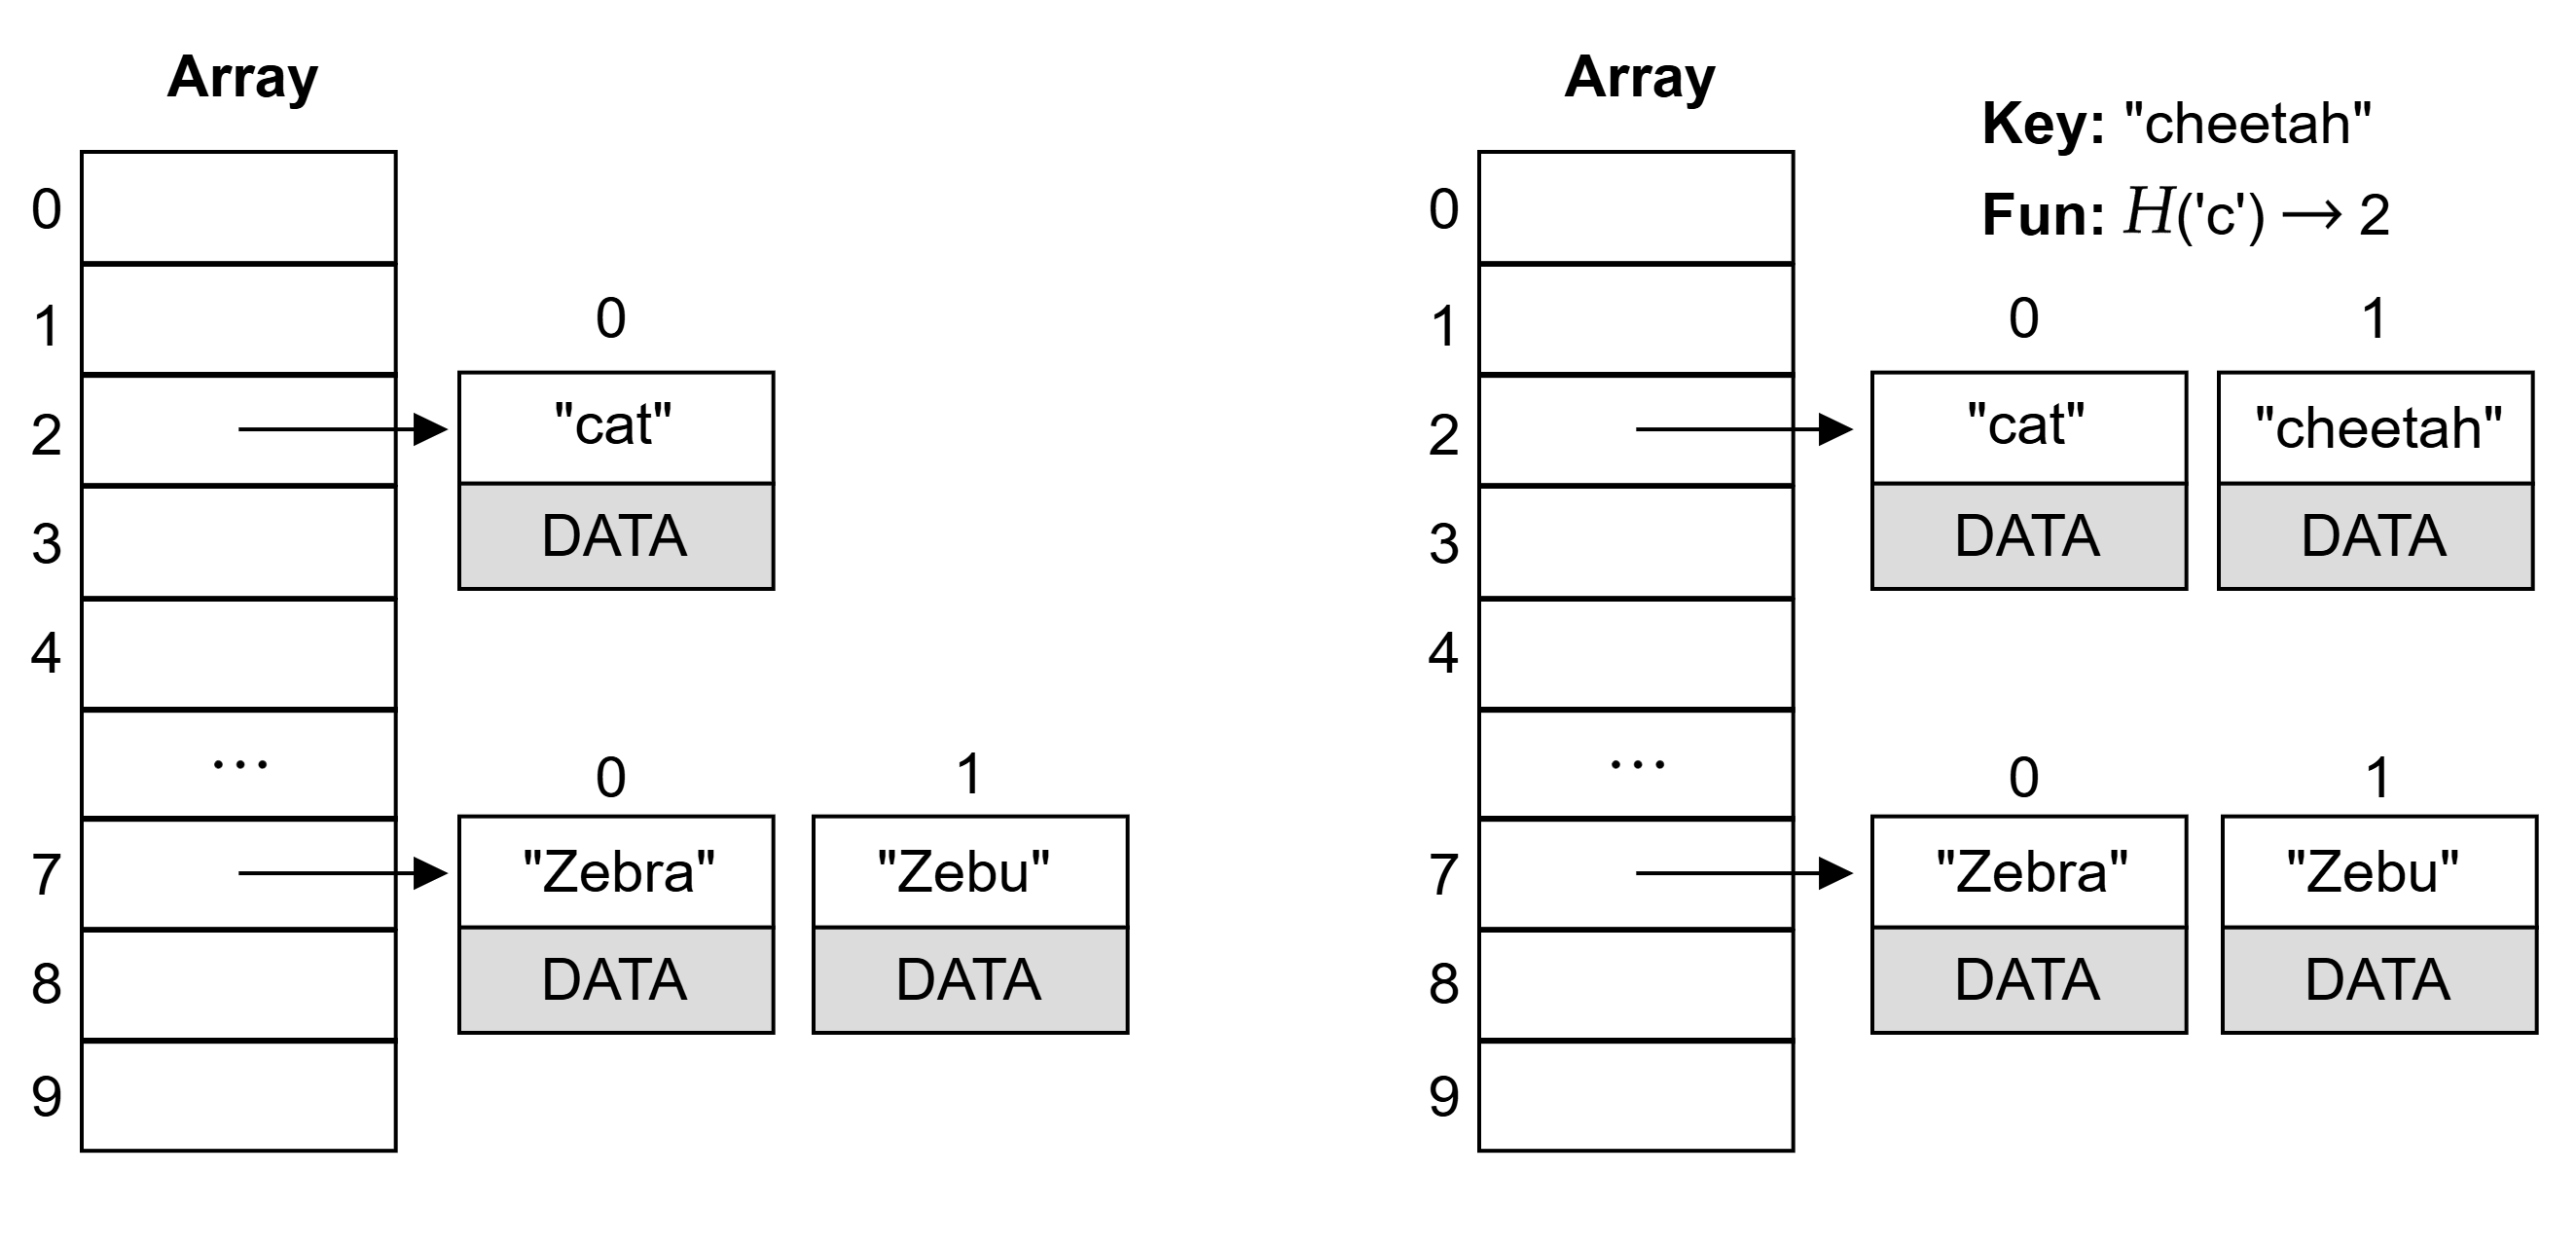
\includegraphics[width=\textwidth]{Sections/hash/separate_chaining.png}
    \caption{The left an array which points to another array (the bucket). The right shows the insertion of 
    ``cheetah'' into the table, indexing at 2, adding to the end of the bucket. Here it's unclear how the data for each element is stored (perhaps a nested array).
    Additionally, the \underline{\textbf{same problem} of resizing} occurs, as if a bucket is another array, we still have to resize it
    (there is no need to rehash the keys in buckets).}
    \label{fig:separate_chaining}
\end{figure}



\begin{Def}[Resizing an Array]

    \label{def:resizing_array}

    Many languages provide a method for resizing an array; However, this is costly as perhaps the next contiguous memory cell 
    for the array is not available in memory. Hence, a new memory region is found and all elements are copied to a new array 
    of larger size, typically $O(n)$, where $n$ is the number of elements in the array.
\end{Def}

\begin{Tip}
    In languages like Java or GO, resizing an array (ArrayList or Slice) is done by creating a new array of double the size and copying all elements over.
\end{Tip}

\newpage 

\noindent
We introduce a new data structure to solve this problem:
\begin{Def}[Linked List]

    A \textbf{linked list} is a data structure consisting of single objects called \textbf{nodes}. Nodes are \emph{linked} together
    via a reference to the next node in the list. This means there are no indices, and the next node can live anywhere
    in memory. The first element is called the \textbf{head}, and the last element is called the \textbf{tail}.
    
    Each node at the very least contains a \textbf{value} and a \textbf{next} pointer to the next node in the list.
    Since a node is an object, an indefinite number of fields can be added to its class definition.
\end{Def}

\begin{Def}[Common Types of Linked Lists]

  
        $\bullet$ \textbf{Singly Linked List:} Each node contains a reference to the next node.\\
        $\bullet$ \textbf{Doubly Linked List:} Each node contains a reference to both the next and previous nodes.\\
        $\bullet$ \textbf{Circular Linked List:} The last node points back to the first node, creating a cycle.

    \noindent
    \rule{\textwidth}{0.4pt}
    \noindent
    \textbf{Time Complexity:} Search is $O(n)$, as we may need to traverse the entire list.
\end{Def}

\begin{figure}[ht!]

    \centering
    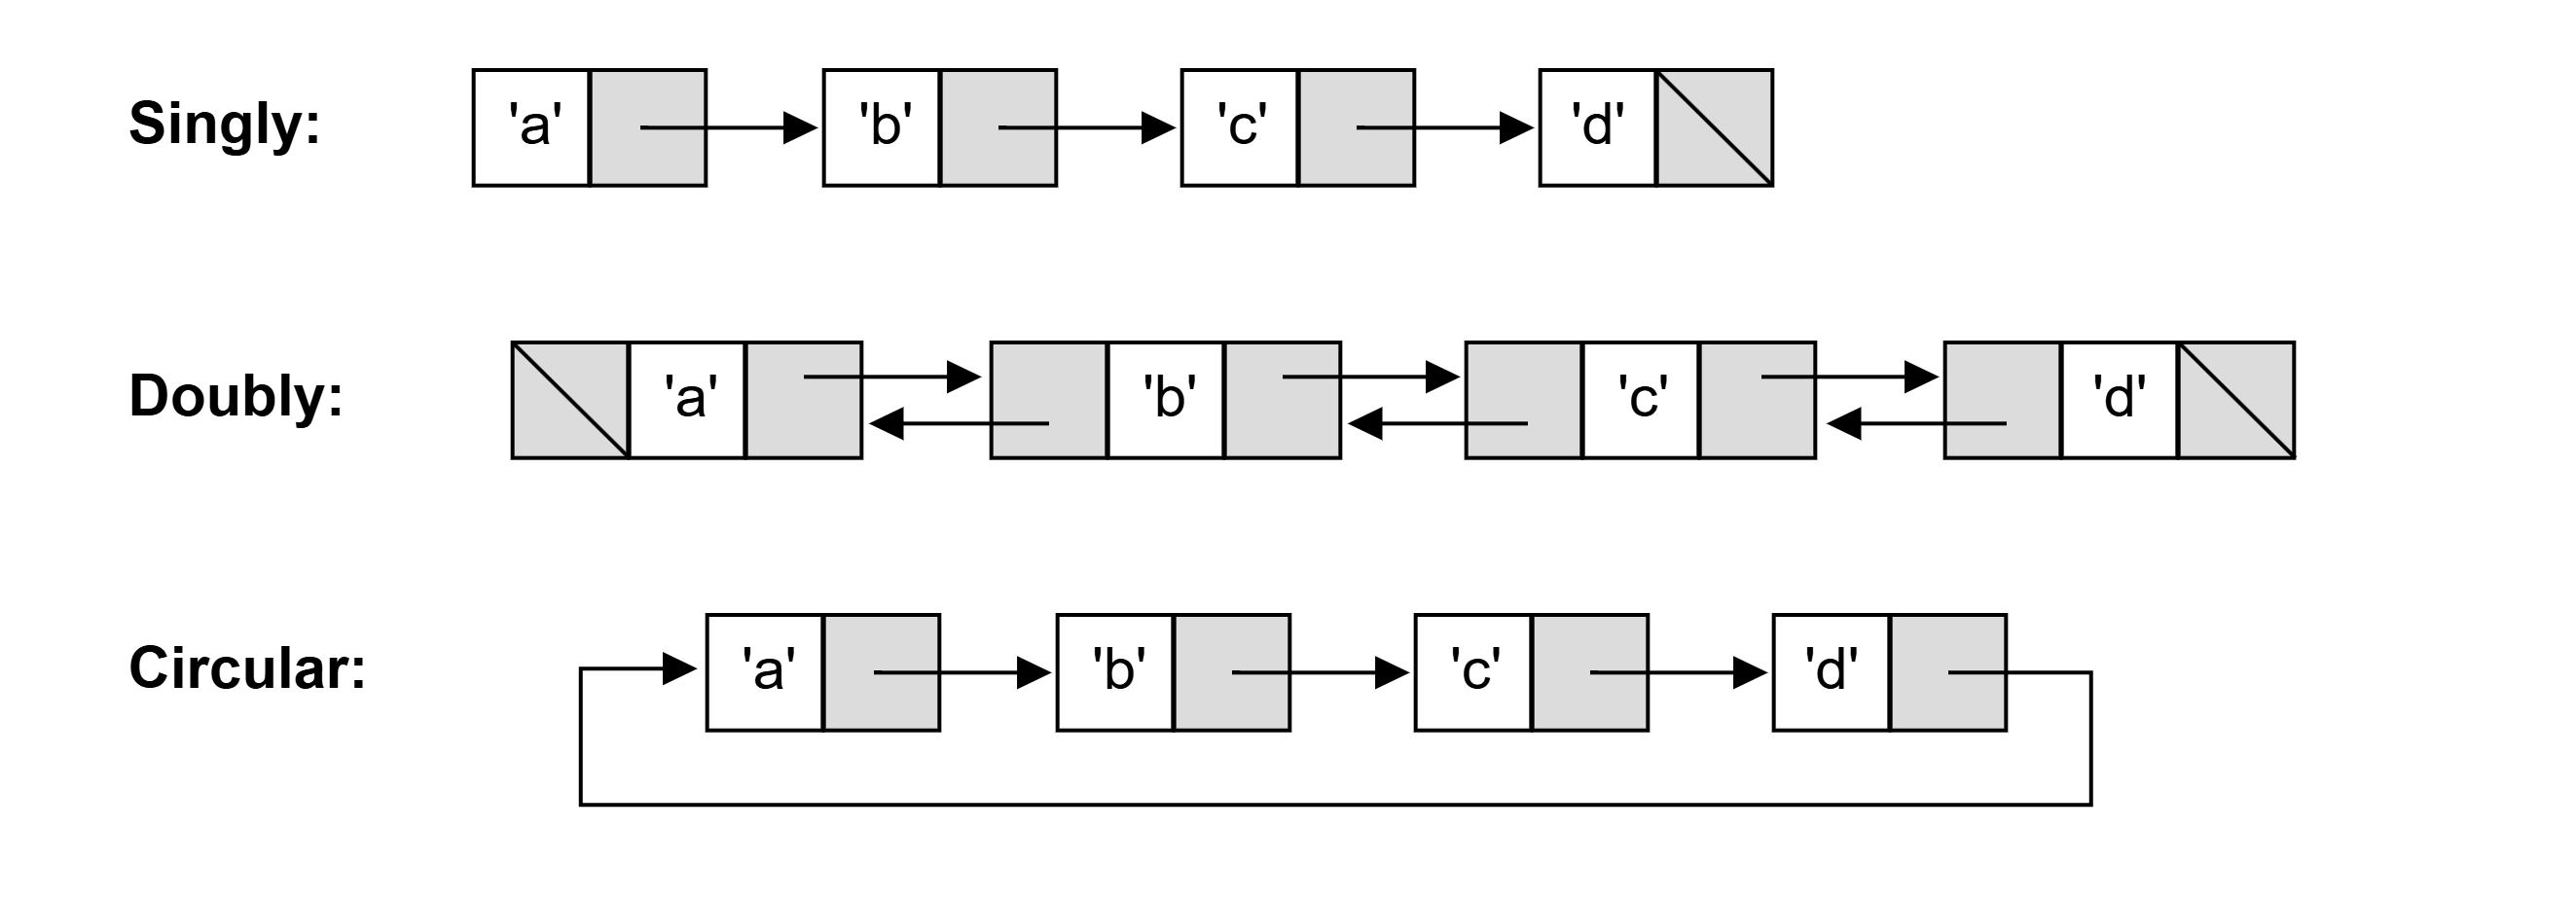
\includegraphics[width=\textwidth]{Sections/hash/linked_list.png}
    \caption{A visual representation of a singly, doubly, and circular linked lists.}
    \label{fig:linked_list}
\end{figure}

\begin{theo}[Open Addressing vs. Separate Chaining]

    \label{thm:open_addressing_vs_separate_chaining}
    
    If updates to the table are \underline{\textbf{rare}} (rehashing on resize), choose open addressing.
    If updates are \underline{\textbf{frequent}}, consider separate chaining.

    It's worth noting that, separate chaining with linked lists requires \textbf{\underline{more memory}} overhead for each node object.
\end{theo}

\newpage
\noindent
We revisit Figure \ref{fig:separate_chaining} with a linked list implementation:

\vspace{-.5em}
\begin{figure}[ht!]

    \centering
    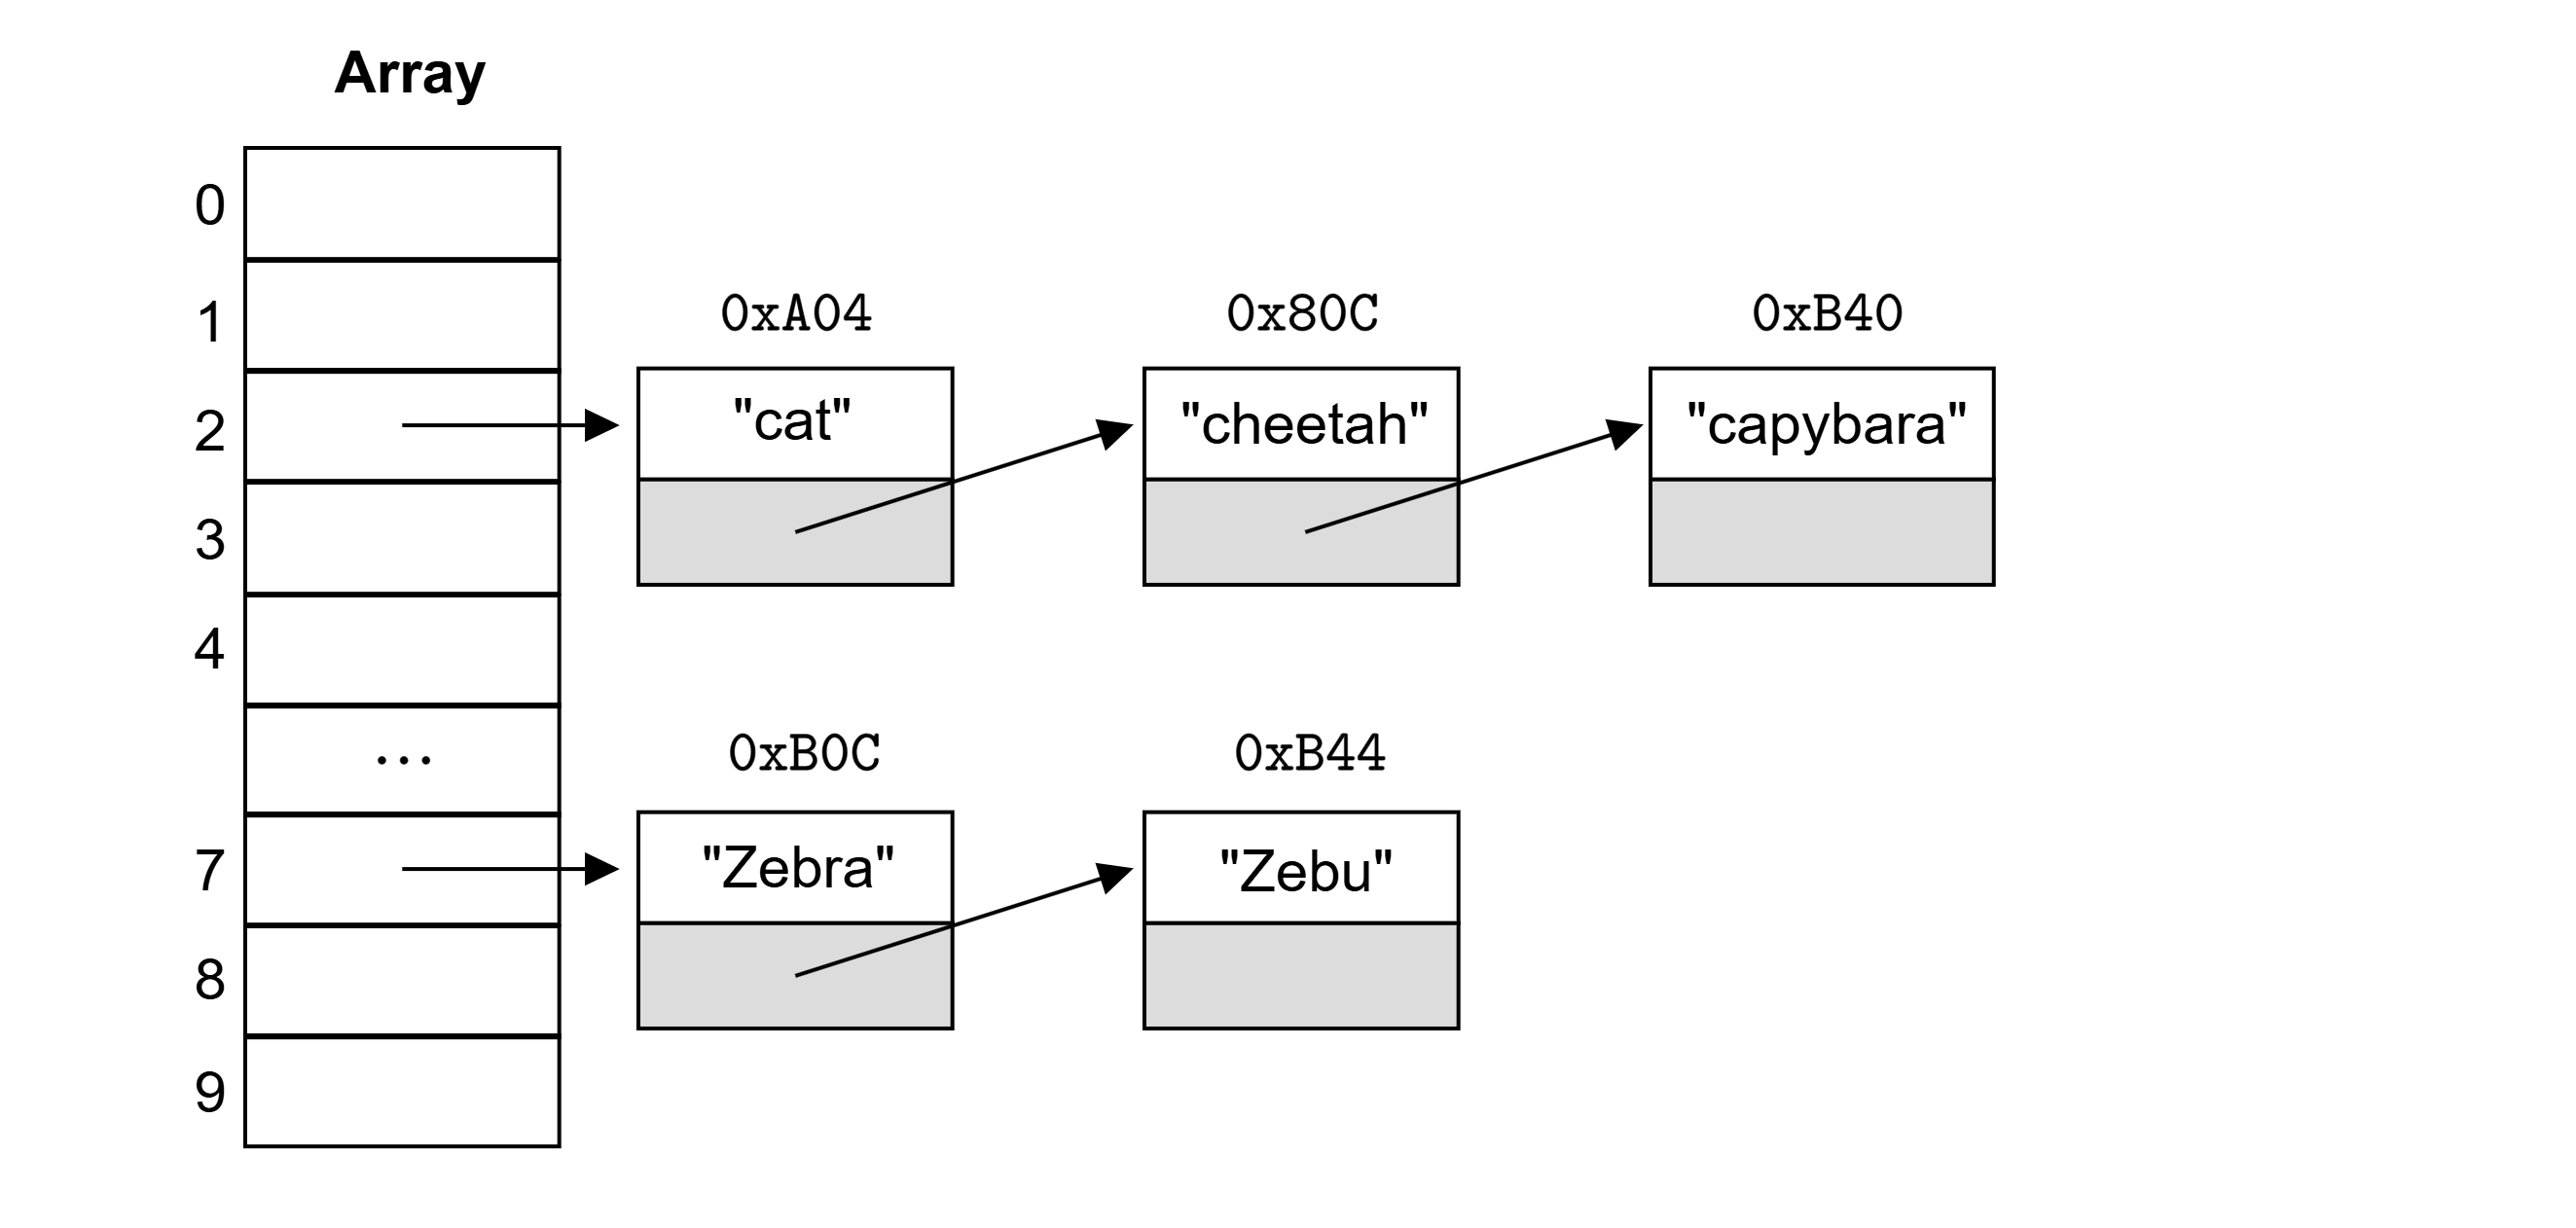
\includegraphics[width=\textwidth]{Sections/hash/separate_chaining_linked_list.png}
    \caption{Here we see an array with two buckets, each bucket is a linked list. Each node points to the next node in 
    the list. In particular, each node lives in at an ambiguous memory location.}
    \label{fig:separate_chaining_linked_list}
\end{figure}

\begin{Def}[Insertion \& Deletion in Linked Lists]

    \label{def:insertion_deletion_linked_list}

    Inserting or deleting relies on shifting pointers around. To make sure references aren't lost to
    the linked list, we always point to a \textbf{dummy head} node, which holds no data and
    always points to the first actual node.

    Say we have two nodes, $A$ and $B$ sequentially in a singly linked list referenced by \texttt{my\_llist} (points to dummy head).
    it has one dot operator, \texttt{my\_llist.next} (the next node in the list).
    \begin{itemize}
        \item \textbf{Inserting:} We attempt to add a new node $C$,
         \begin{itemize}
            \item \textbf{At the head:} Set \texttt{my\_llist.next = C} and \texttt{C.next = A}, $O(1)$.
            \item \textbf{At the tail:} Traverse the list until via \texttt{my\_llist.next} until a null \texttt{.next}
            is found, set the previous node's \texttt{.next} to $C$ and \texttt{C.next = null}, $O(n)$.
            \item \textbf{In the middle:} Traverse the list until node $A$ is found,
            set \texttt{C.next = A.next}, then \texttt{A.next = C.next}, $O(n)$.
        \end{itemize}
        \item \textbf{Deleting:} Now we have three sequential nodes, $A$, $B$, and $C$.
        \begin{itemize}
            \item \textbf{The head:} Set \texttt{my\_llist.next = A.next}, discards references to $A$, $O(1)$.
            \item \textbf{The tail:} Traverse and set \texttt{B.next = null}, $O(n)$ (discards $C$).
            \item \textbf{In the middle:} Traverse and set \texttt{A.next = B.next}, $O(n)$ (discards $B$).
        \end{itemize}
    \end{itemize}
\end{Def}
\noindent
Visualizations on the next page.

\newpage 

\begin{Example}[Insertion \& Deletion in Linked Lists -- Corollary]

    If we know the position of the node to be inserted or deleted, we can directly access it via a pointer. Revisiting 
    Definition \ref{def:insertion_deletion_linked_list}, we can insert or delete in constant time $O(1)$, instead of traversing the list.
    To demonstrate deletion, we have three sequential nodes, $A$, $B$, and $C$:

    \begin{itemize}
        \item \textbf{The head:} Set \texttt{my\_llist.next = my\_llist.next.next}, discards references to $A$.
        \item \textbf{The tail:} Set \texttt{my\_llist.next.next.next = null}, discards $C$.
        \item \textbf{In the middle:} Set \texttt{my\_llist.next.next = my\_llist.next.next.next}, discards $B$.
    \end{itemize}

    \noindent
    This is a bit hard to read, we visualize it as follows:

    \begin{center}
    
    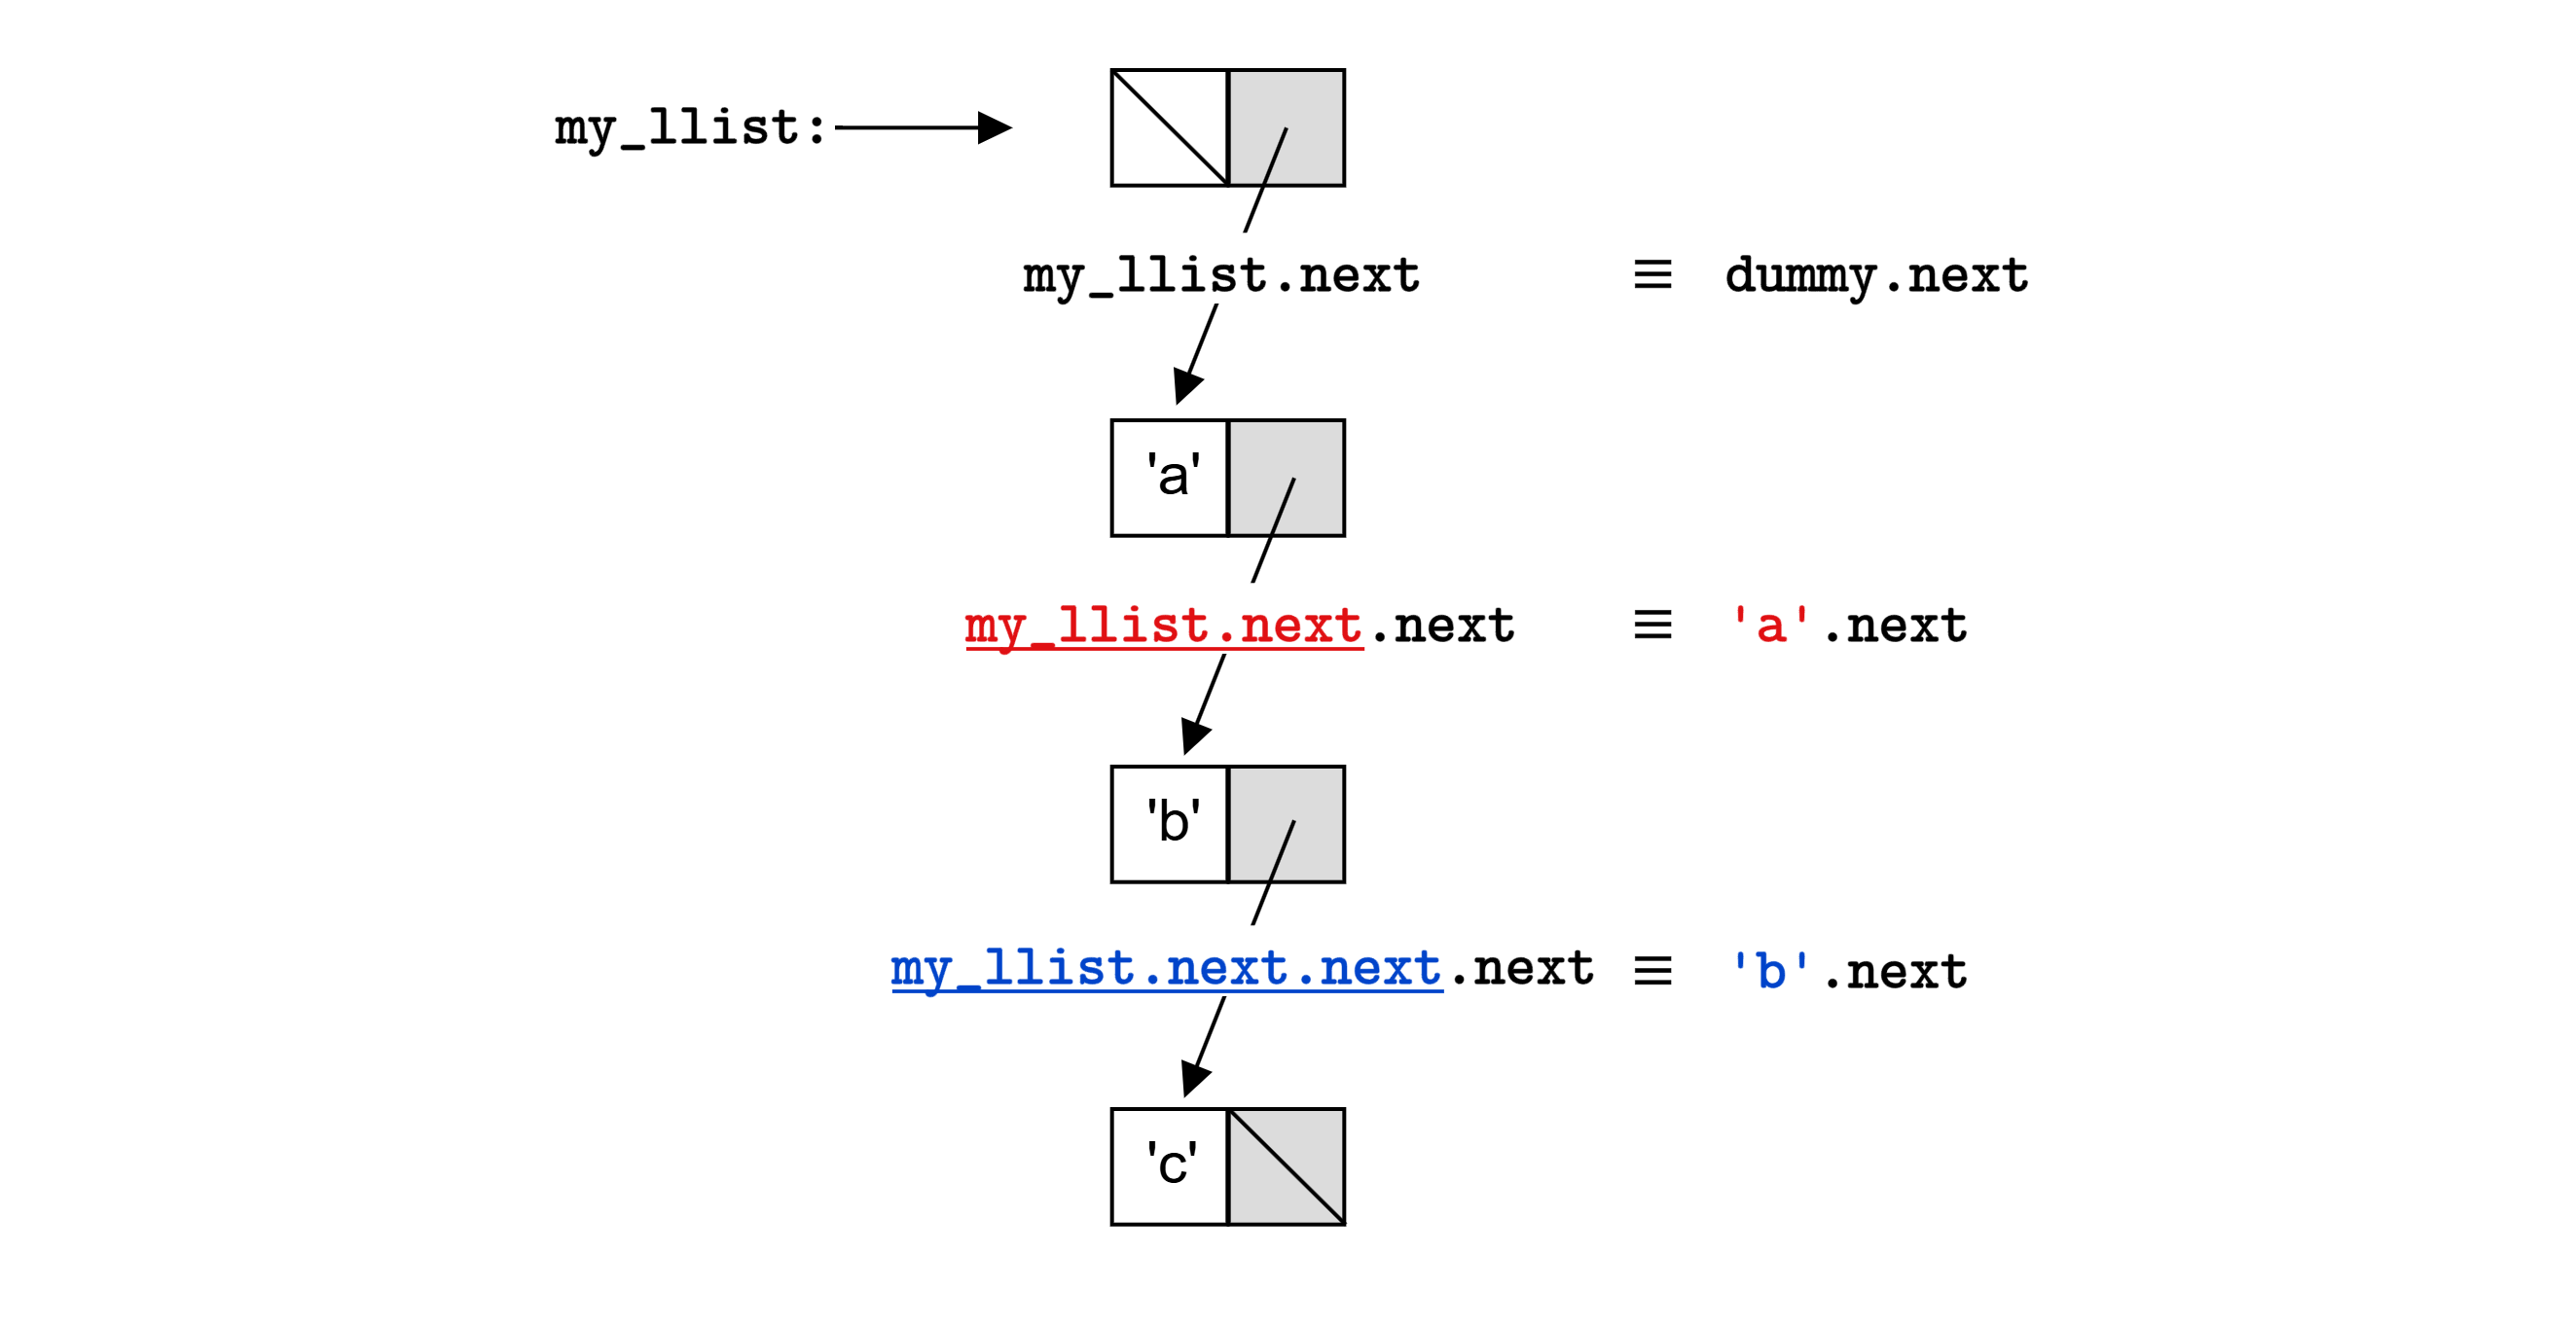
\includegraphics[width=\textwidth]{Sections/hash/llist_dots.png}
    \end{center}

    \noindent
    In other words, \texttt{my\_llist} is the dummy head node, \texttt{my\_llist.next} returns the dummy node's \texttt{next} pointer (an address). 
    If we \emph{act} on such address, we access the address's fields. Hence, \texttt{my\_llist.next.next} $\equiv$ \texttt{A.next}. Again,
    \texttt{A.next} $\equiv$ \texttt{B} (the address). So,
    \begin{align*}
        \texttt{my\_llist.next.next.next} &\equiv \texttt{A.next.next} \\
        &\equiv \texttt{B.next} \\
        &\equiv \texttt{C} \quad \text{(the address)}
    \end{align*}

    \noindent
    Still, it's not advisable to code like this, primarily because of readability.
\end{Example}

\newpage

\subsection{Load Factor \& Performance Metrics}

\noindent
We want to be pre-emptive at avoiding collisions and resizing the table. The following measurement tracks this:

\begin{Def}[Load Factor]

    \label{def:load_factor}

    The \textbf{load factor} \(\alpha\) of a hash table is defined as the ratio of the number of elements \(n\) to the size of the table \(m\):
    \[
        \alpha :=  \frac{n}{m}
    \]

    \begin{itemize}
        \item \textbf{Open Addressing:} $\alpha < 0.5$.
        \item \textbf{Separate Chaining:} $\alpha < 1$.
    \end{itemize}

    \noindent
    Once $\alpha$ exceeds the optimal threshold, we should \textbf{consider resizing} the table. Upon good load conditions, we
    generally expect $\Theta(1)$ and $\Theta(1 + \alpha)$ time complexity for insertion and deletion, respectively with open addressing and separate chaining.
\end{Def}

\begin{table}[ht!]
    \centering
    \begin{tabular}{l|c|c}
        \hline
        Method & Insertion & Deletion \\
        \hline
        Open Addressing       & \(\Theta (1)\) average, \(O(n)\) worst & \(\Theta (1)\) average, \(O(n)\) worst \\
        Separate Chaining     & \(\Theta(1 + \alpha)\) average, \(O(n)\) worst & \(\Theta(1 + \alpha)\) average, \(O(n)\) worst \\
        \hline
    \end{tabular}
    \caption{Time-complexity comparison of insertion and deletion in open addressing vs.\ separate chaining (where \(\alpha\) is the load factor).}
    \label{tab:hash_complexities}
\end{table}

\begin{table}[ht!]
    \centering
    \begin{tabular}{l|c|c}
        \hline
        \textbf{Operation}      & \textbf{Dynamic Array}       & \textbf{Singly Linked List} \\ \hline
        Insert at head          & $O(n)$ (shift all elements) & $O(1)$                       \\
        Insert at tail          & $O(1)$                       & $O(n)$                       \\
        Insert in middle        & $O(n)$                        & $O(n)$                       \\ \hline
        Delete at head          & $O(n)$                        & $O(1)$                       \\
        Delete at tail          & $O(1)$                        & $O(n)$                       \\
        Delete in middle        & $O(n)$                        & $O(n)$                       \\ \hline 
        Search for element      & $O(n)$                        & $O(n)$                       \\
        Random access           & $O(1)$                        & $O(n)$ (traversal)           \\
    \end{tabular}
    \caption{Inserting or deleting elements in dynamic arrays (growing) versus singly linked lists. In particular,
    maintaining order within a dynamic array forces shifting of elements upon insertion or deletion.}

\end{table}